\documentclass{article}[18pt]
\usepackage{../../../format}
\lhead{A Level Physics - Further Mechanics and Thermal Physics}

%File specific Preamble
\usepackage{tabu} %Table

\pgfkeys{/pgfplots/Axis Style/.style={
    width=13.5cm, height=5cm,
    axis x line=center, 
    axis y line=middle, 
    samples=100,
    ymin=-1.5, ymax=1.5,
    xmin=0, xmax=14.0,
    domain=-4*pi:4*pi
}}

%Diagram
\pgfdeclarelayer{background layer}
\pgfdeclarelayer{foreground layer}
\pgfsetlayers{background layer,main,foreground layer}

\begin{document}
\begin{center}
\underline{\huge Simple Harmonic Motion}
\end{center}

\section{Introduction}
An object is undergoing Simple harmonic motion if:
\begin{itemize}
\item Its acceleration is proportional to its displacement.
\item Acceleration is directed to the equilibrium point (in the opposite direction to the displacement.
\end{itemize}

Rules of simple harmonic motion:
\begin{itemize}
\item The object can't have frictional forces (no damping)
\item The oscillations must be small displacements
\end{itemize}



\begin{tikzpicture}
\begin{axis}[
    Axis Style,
    xtick={
        3.14159,6.28319,9.42478,12.56637
    },
    xticklabels={
        $\dfrac{T}{2}$,T,$\dfrac{3T}{2}$,2T
    },
    ytick={-1,1},
    yticklabels={-A,A},
    y label style={at={(axis description cs:-0.1,.5)},rotate=90,anchor=south},
    ylabel = {Displacement, x},
    xlabel= {Time, t}
]
\addplot [mark=none, ultra thick, black] {cos(deg(x))};
\end{axis}
\end{tikzpicture}
$x=Acos(\omega t)$
\\
\begin{tikzpicture}
\begin{axis}[
    Axis Style,
    xtick={
        3.14159,6.28319,9.42478,12.56637
    },
    xticklabels={
        $\dfrac{T}{2}$,T,$\dfrac{3T}{2}$,2T
    },
    ytick={-1,1},
    yticklabels={$-\omega A$,$\omega A$},
    y label style={at={(axis description cs:-0.1,.5)},rotate=90,anchor=south},
    ylabel = {Velocity, v},
    xlabel= {Time, t}
]
\addplot [mark=none, ultra thick, black] {-sin(deg(x))};
\end{axis}
\end{tikzpicture}
$v=-\omega A\sin(\omega t)$
\\
\begin{tikzpicture}
\begin{axis}[
    Axis Style,
    xtick={
        3.14159,6.28319,9.42478,12.56637
    },
    xticklabels={
        $\dfrac{T}{2}$,T,$\dfrac{3T}{2}$,2T
    },
    ytick={-1,1},
    yticklabels={$-\omega^2 A$,$\omega^2 A$},
    y label style={at={(axis description cs:-0.1,.5)},rotate=90,anchor=south},
    ylabel = {Acceleration, a},
    xlabel= {Time, t}
]
\addplot [mark=none, ultra thick, black] {-cos(deg(x))};
\end{axis}
\end{tikzpicture}
$a=-\omega^2A\cos(\omega t)$
\section{Acceleration vs Displacement SHM Graph}
\begin{tikzpicture}[scale=0.7]
\begin{axis}[axis lines=middle,xtick={-4,4},xticklabels={-A,A},ytick={-4,4},yticklabels={$-\omega^2A$,$\omega^2A$},
ylabel=a/$ms^{-2}$,y label style={at={(ticklabel* cs:1.1)},anchor=north},
xlabel=x/m,x label style={at={(ticklabel* cs:1.1)},anchor=east}
]
\addplot[domain=-4:4]{-x};
\end{axis}
\end{tikzpicture}
\newpage
\section{Period of a pendulum}
$T=2\pi\sqrt{\dfrac{L}{g}}$\\
$T^2=\dfrac{4\pi^2L}{g}$\\
\begin{tikzpicture}[scale=0.5]
\begin{axis}[ymin=-0.01,ticks=none,ylabel=$T^2/s^2$,xlabel=$L/m$,axis lines=middle,label style={font=\large}]
\addplot[mark=none]{x};
\end{axis}
\end{tikzpicture}\\
The gradient of the graph is $\dfrac{4\pi^2}{g}$\\
\section{Energy in SHM}
\begin{tikzpicture}
\begin{axis}[
    Axis Style,
    xtick={
        3.14159,6.28319
    },
    xticklabels={
        $\dfrac{T}{2}$,T
    },
    ytick={1},
    yticklabels={$\frac{1}{2}m\omega^2A^2$},
    y label style={at={(axis description cs:-0,.25)},rotate=90,anchor=south},
    ylabel = {Energy/J},
    xlabel= {Time, t},
    x label style={at={(axis description cs:1.12,0)},anchor=east},
    xmax=6.28319,
    ymin=0
]
\addplot [mark=none, ultra thick, black,samples=200] {(cos(deg(x)))^2};
\addplot [mark=none, ultra thick, red,samples=200] {(sin(deg(x)))^2};
\end{axis}
\end{tikzpicture}
\\
Red - Kinetic Energy\\
Black - Gravitational potential energy\\
\\
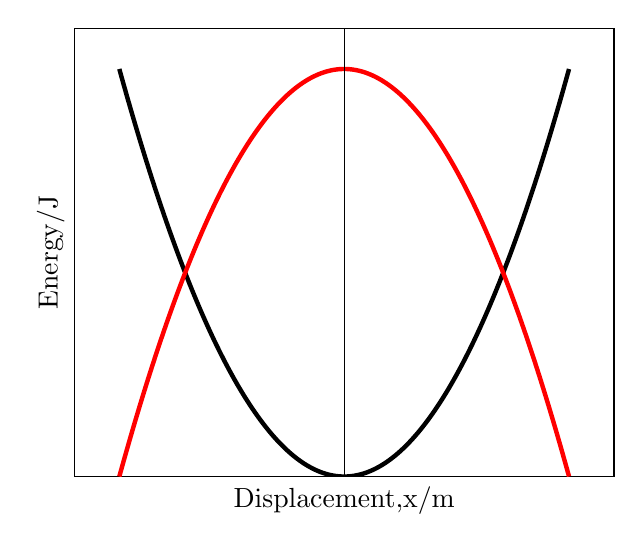
\begin{tikzpicture}
\begin{axis}[ymin=0,ticks=none,xlabel={Displacement,x/m},ylabel={Energy/J}]
\addplot [mark=none, ultra thick, black,samples=200] {x^2};
\addplot [mark=none, ultra thick, red,samples=200] {-x^2+25};
\draw[ultra thin] (axis cs:0,\pgfkeysvalueof{/pgfplots/ymin}) -- (axis cs:0,\pgfkeysvalueof{/pgfplots/ymax});
\end{axis}
\end{tikzpicture}
\newpage
\section{Barton's Pendulum}

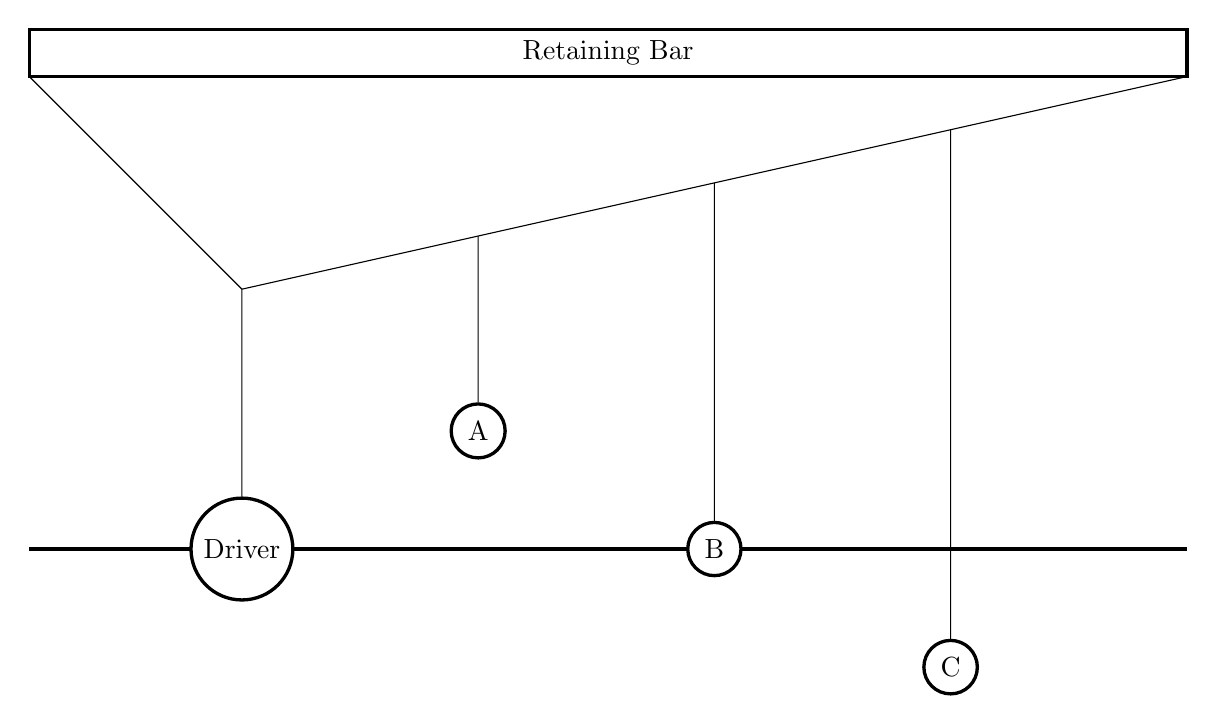
\begin{tikzpicture}[scale=0.3,
bob/.style={circle, draw=black, fill=white, very thick, minimum size=5mm}
]
\draw[black, very thick] (0,0)rectangle (49,2) node[pos=.5] {Retaining Bar};
\draw (0,0) -- (9,-9);
\draw (9,-9) -- (49,0);
\node[bob] (driver) at (9,-20) {Driver};
\draw (9,-9) -- (driver.north);
\node[bob] (a) at (19,-15) {A};
\draw (19,-6.75) -- (a.north);
\node[bob] (b) at (29,-20) {B};
\draw (29,-4.5) -- (b.north);
\node[bob] (c) at (39,-25) {C};
\draw (39,-2.25) -- (c.north);
\begin{pgfonlayer}{background layer}
\draw[very thick] (0,-20) -- (49,-20);
\end{pgfonlayer}{background layer}
\end{tikzpicture}
\\
\\
All lengths are measured from the retaining bar to the centre of mass of the bob.\\
\\
The \textbf{natural} frequency is the frequency of an object oscillating in the absence of any driving or damping force \textbf{Driver in diagram}.\\
\\
The \textbf{driven} frequency is where an external force is provided, making the oscillator undergo forced vibrations. \textbf{A,B and C in diagram}.\\
\\
\textbf{Resonance} occurs when the frequency of the driving force is equal to the natural frequency and can result in large amplitude oscillations. \textbf{B in diagram}.\\
\\



\begin{tabu} to \textwidth { | X[c] | X[c] | X[c] | X[c] | }
 \hline
\textbf{Pendulum}&\textbf{Natural frequency}&\textbf{Amplitude(wrt driver)}&\textbf{Phase(wrt driver)} \\
\hline
A&Higher than driver&Small&In phase\\
\hline
B&Equal to driver (resonance)&Large&Out of phase$(90\degree or \frac{\pi}{2})$\\
\hline
C&Lower than driver&Smaller than resonant&Antiphase$(180\degree or \pi)$\\
\hline
\end{tabu}


\section{How do engineers prevent resonance}
Ways to prevent resonance
\begin{itemize}
\item Use several materials - they all have different resonance properties
\item Don't have symmetry - prevents standing waves
\item Use very stiff materials - High frequency, small wavelengths
\end{itemize}


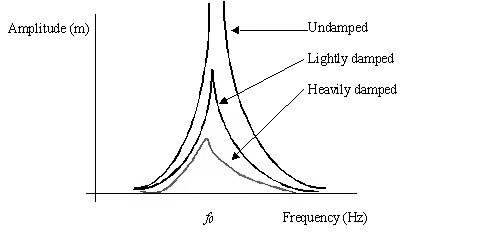
\includegraphics[width=7cm] {damp_6.jpg}
\section{Damping}
Damping is the reduction in amplitude due to energy losses (e.g. overcoming friction).\\
\\
It will also cause the period to increase (it is essentially a driver).\\
\\
\textbf{Light(underdamping)} - Small amplitude change per oscillation\\
\textbf{Heavy(underdamping)} - Large amplitude change per oscillation\\
\\
\textbf{Critical damping} - Reaches equilibrium in the shortest possible time \textbf{without} oscillating\\
\\
\textbf{Over damping} - Reaches equilibrium after a long period of time
\subsection{Damping graph}
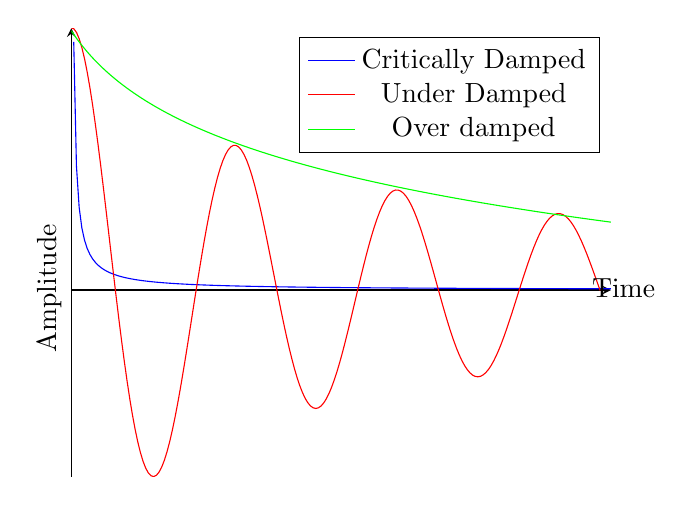
\begin{tikzpicture}
\begin{axis}[axis lines=middle,samples=200,ymax=10,ticks=none,ylabel=Amplitude,ylabel style={rotate=90, anchor=south,at={(axis description cs:0,0.42)},},xlabel=Time,x label style={at={(axis description cs:1.1,0.42)},anchor=east},]
\addplot[blue,domain=0:21] {1/x};\addlegendentry{Critically Damped}
\addplot[red,domain=0.01:20.58] {78*sin(deg(x+7.7))/(x+7.7)};\addlegendentry{Under Damped}
\addplot[green,domain=0.01:21] {-3*ln(x+2)+12};\addlegendentry{Over damped}
\end{axis}
\end{tikzpicture}
\section{Mass spring system}
\subsection{Period of a mass-spring system}
The period of a mass-spring system is $T=2\pi\sqrt{\dfrac{m}{k}}$ or $T^2=\dfrac{4\pi^2m}{k}$\\
\begin{tikzpicture}[scale=0.5]
\begin{axis}[ymin=-0.001,ticks=none,ylabel=$T^2/s^2$,xlabel=$m/kg$,axis lines=middle,
label style={font=\large}
]
\addplot[mark=none]{x};
\end{axis}
\end{tikzpicture}\\
The gradient is $\dfrac{4\pi^2}{k}$\\
The line passes through the origin\\
This is only true for small oscillations as large oscillations go past the limit of proportionality
\subsection{Energy in a vertically oscillating spring}
\begin{tabular}{|c|c|c|c|}
\hline
&KE&GPE&Elastic Energy\\
\hline
Top&0&$2mgA$&$\frac{1}{2}k(e-A)^2$\\
\hline
Middle&Max=$\frac{1}{2}m\omega^2A^2$&$mgA$&$\frac{1}{2}ke^2$\\
\hline
Bottom&0&0&$\frac{1}{2}k(e+A)^2$\\
\hline
\end{tabular}






\end{document}